% Game state machine, from final_report.tex (fig:states), recoloured for the slides.
\documentclass[border=4pt]{standalone}
% Shared look for the slide diagrams: the deck's dark colours, sans text, transparent background.
\usepackage[scaled]{helvet}
\renewcommand{\familydefault}{\sfdefault}
\usepackage{tikz}
\usetikzlibrary{arrows.meta,positioning,fit,calc}
\definecolor{fg}{HTML}{F3F1EA}
\definecolor{muted}{HTML}{C9D2DC}
\definecolor{card}{HTML}{1A2430}
\definecolor{fin}{HTML}{243142}
\definecolor{edge}{HTML}{8C98A5}
\definecolor{amber}{HTML}{F5A524}
\definecolor{bg}{HTML}{111821}
\color{fg}

\begin{document}
\color{fg}
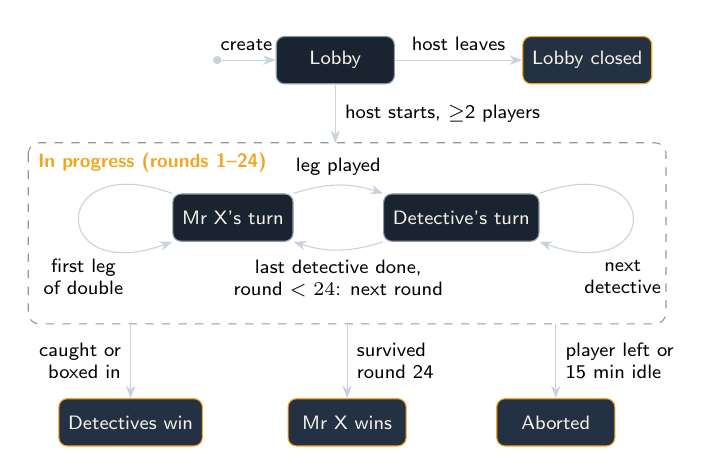
\begin{tikzpicture}[
  font=\scriptsize,
  st/.style={draw=edge, rounded corners=3pt, align=center, minimum height=6mm, minimum width=15mm, fill=card, text=fg},
  fin/.style={st, fill=fin, draw=amber},
  arr/.style={-{Stealth[length=1.6mm]}, draw=muted}]
  \node[st] (lobby) at (0,0) {Lobby};
  \node[fin] (closed) at (3.2,0) {Lobby closed};
  \node[st] (mrx) at (-1.3,-2.0) {Mr~X's turn};
  \node[st] (det) at (1.6,-2.0) {Detective's turn};
  \draw[dashed, draw=edge, rounded corners=4pt] (-3.9,-1.05) rectangle (4.2,-3.35);
  \node[font=\scriptsize\bfseries, anchor=north west, text=amber] at (-3.9,-1.05) {In progress (rounds 1--24)};
  \node[fin] (dw) at (-2.6,-4.6) {Detectives win};
  \node[fin] (xw) at (0.15,-4.6) {Mr~X wins};
  \node[fin] (ab) at (2.8,-4.6) {Aborted};
  \fill[muted] (-1.5,0) circle (1.5pt) coordinate (s);
  \draw[arr] (s) -- node[above]{create} (lobby);
  \draw[arr] (lobby) -- node[above]{host leaves} (closed);
  \draw[arr] (lobby.south) -- node[right, align=left]{host starts, $\geq$2 players} (0,-1.05);
  \draw[arr] (mrx.north east) to[bend left=18] node[above]{leg played} (det.north west);
  \draw[arr] (det.south west) to[bend left=18] node[below, align=center]{last detective done,\\round $<24$: next round} (mrx.south east);
  \draw[arr] (mrx.north west) to[out=160, in=200, looseness=7] (mrx.south west);
  \node[align=center] at (-3.2,-2.75) {first leg\\of double};
  \draw[arr] (det.north east) to[out=20, in=-20, looseness=7] (det.south east);
  \node[align=center] at (3.65,-2.75) {next\\detective};
  \draw[arr] (dw.north |- 0,-3.35) -- node[left, align=right]{caught or\\boxed in} (dw);
  \draw[arr] (xw.north |- 0,-3.35) -- node[right, align=left]{survived\\round 24} (xw);
  \draw[arr] (ab.north |- 0,-3.35) -- node[right, align=left]{player left or\\15 min idle} (ab);
\end{tikzpicture}
\end{document}
